\documentclass[xcolor=dvipsnames]{beamer}
\usepackage[T1]{fontenc}
\usepackage[utf8]{inputenc}
\usepackage[english,slovak]{babel}

\usepackage{amsmath}
\usepackage{amsthm}
\usetheme{Pittsburgh}
\useoutertheme{shadow}

\usepackage{graphicx}
\usepackage{caption}
\usepackage{subcaption}

\usepackage[]{algorithm2e}
\usepackage{listings}
 \setbeamercovered{transparent}
 \usepackage{cuted}
\usepackage[export]{adjustbox}
\usepackage{mathtools}

\usepackage{lipsum}
\usepackage{verbatim}
\usepackage{transparent}
\usepackage{framed}
\usepackage{xcolor}

\usepackage{multirow}
\usepackage{colortbl}
\usepackage{lmodern}

\usepackage{animate,media9,movie15}

\newcommand\Wider[2][3em]{%
\makebox[\linewidth][c]{%
  \begin{minipage}{\dimexpr\textwidth+#1\relax}
  \raggedright#2
  \end{minipage}%
  }%
}




\iffalse

\usetheme{Warsaw}

\setbeamercolor{normal text}{fg=white,bg=black!90}
\setbeamercolor{structure}{fg=white}

\setbeamercolor{alerted text}{fg=red!85!black}

\setbeamercolor{item projected}{use=item,fg=black,bg=item.fg!35}

\setbeamercolor*{palette primary}{use=structure,fg=structure.fg}
\setbeamercolor*{palette secondary}{use=structure,fg=structure.fg!95!black}
\setbeamercolor*{palette tertiary}{use=structure,fg=structure.fg!90!black}
\setbeamercolor*{palette quaternary}{use=structure,fg=structure.fg!95!black,bg=black!80}

\setbeamercolor*{framesubtitle}{fg=white}

\setbeamercolor*{block title}{parent=structure,bg=black!60}
\setbeamercolor*{block body}{fg=black,bg=black!10}
\setbeamercolor*{block title alerted}{parent=alerted text,bg=black!15}
\setbeamercolor*{block title example}{parent=example text,bg=black!15}

\fi



%-------------------------------------------------------------------------------------
\title{\color{white} \bf Deep learning}
\author{\color{white} Michal CHOVANEC, PhD}


%\setbeamertemplate{footline}[frame number]{}
\setbeamertemplate{navigation symbols}{}


\date[EURP]{}
\begin{document}

{
    \usebackgroundtemplate
    {
        \vbox to \paperheight{\vfil\hbox to \paperwidth{\hfil

        {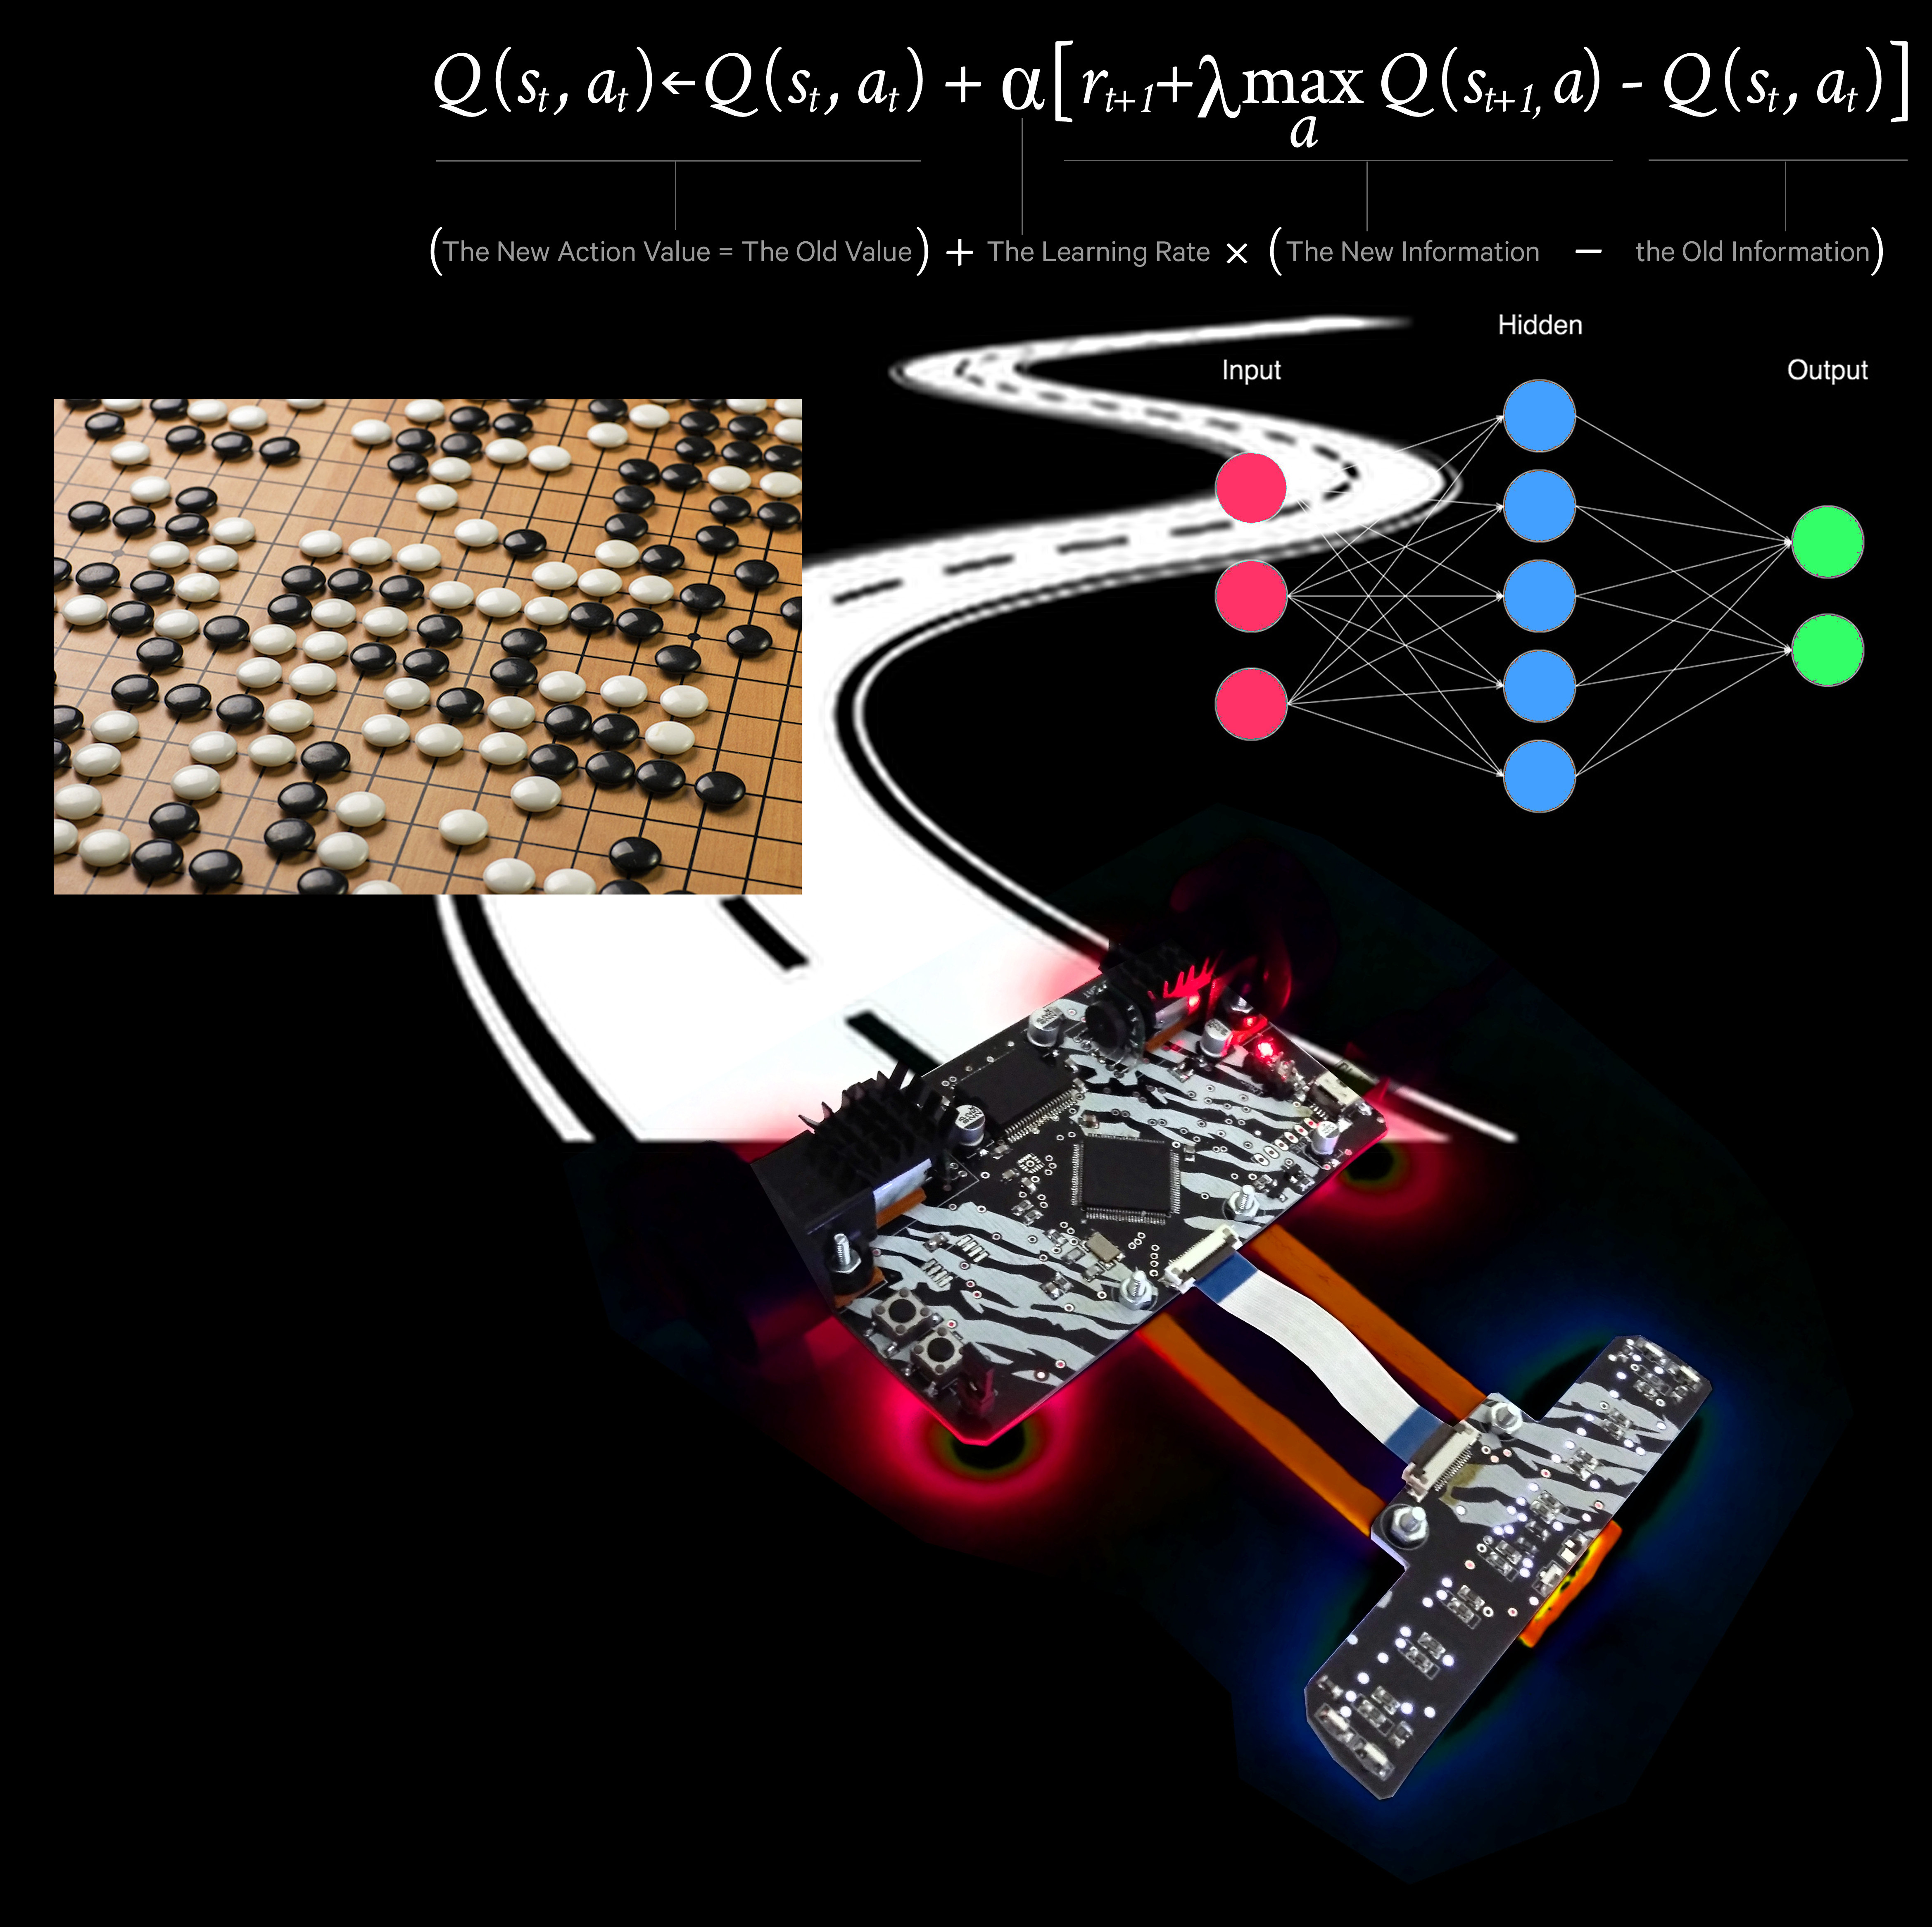
\includegraphics[width=5.05in]{../../pictures/rl_square.jpg}}

        \hfil}\vfil}
    }
    \begin{frame}

    %\titlepage


    \centering
     \colorbox{black}
     {
        \begin{minipage}{7cm}
           {\LARGE \color{white} \bf Deep learning} \\
           {\LARGE \color{white} Michal CHOVANEC, PhD} \\
       \end{minipage}
     }


    \end{frame}
}


\begin{frame}{\bf Playing Atari games on super human level}

\begin{columns}

    \begin{column}{0.5\textwidth}

        \includemovie[
          poster,
          autoplay,
          externalviewer,
          inline=false,
          text={\small(video)}
        ]{4cm}{4cm}{../../video/rl_arkanoid_05.mp4}

        \begin{figure}
        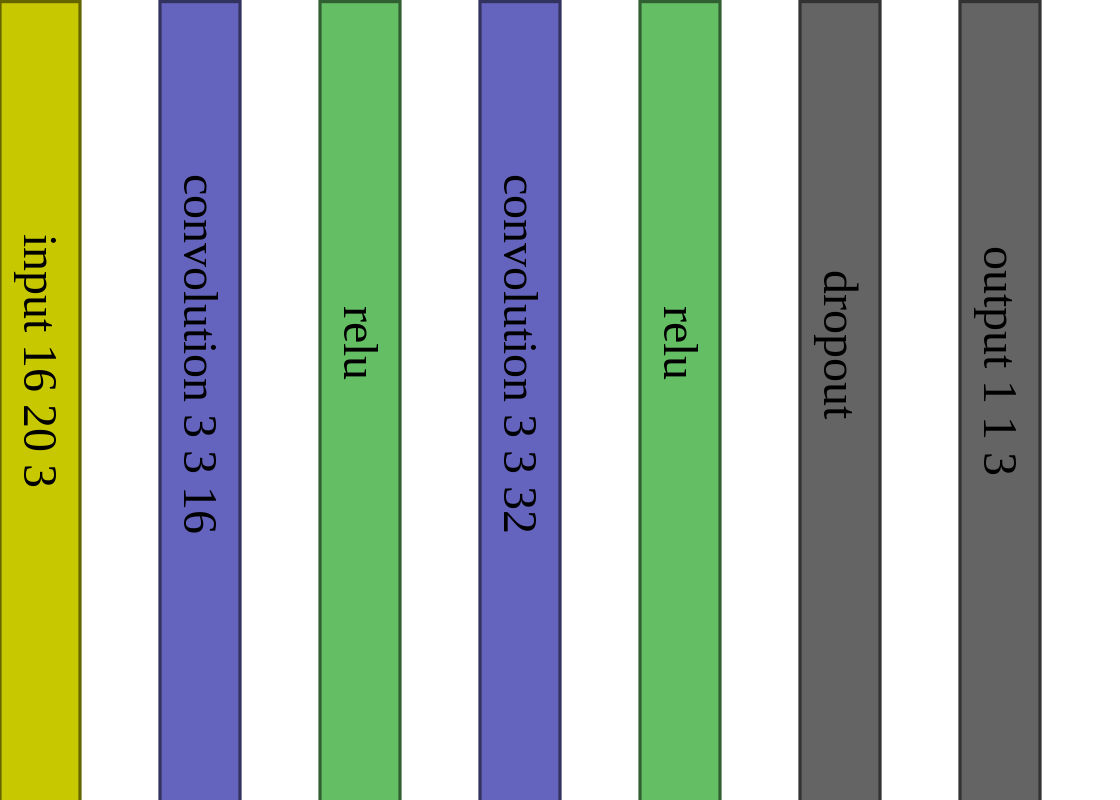
\includegraphics[scale=0.12]{../../diagrams/arkanoid_net.png}
        \end{figure}

    \end{column}

    \begin{column}{0.5\textwidth}  %%<--- here

        \begin{figure}
          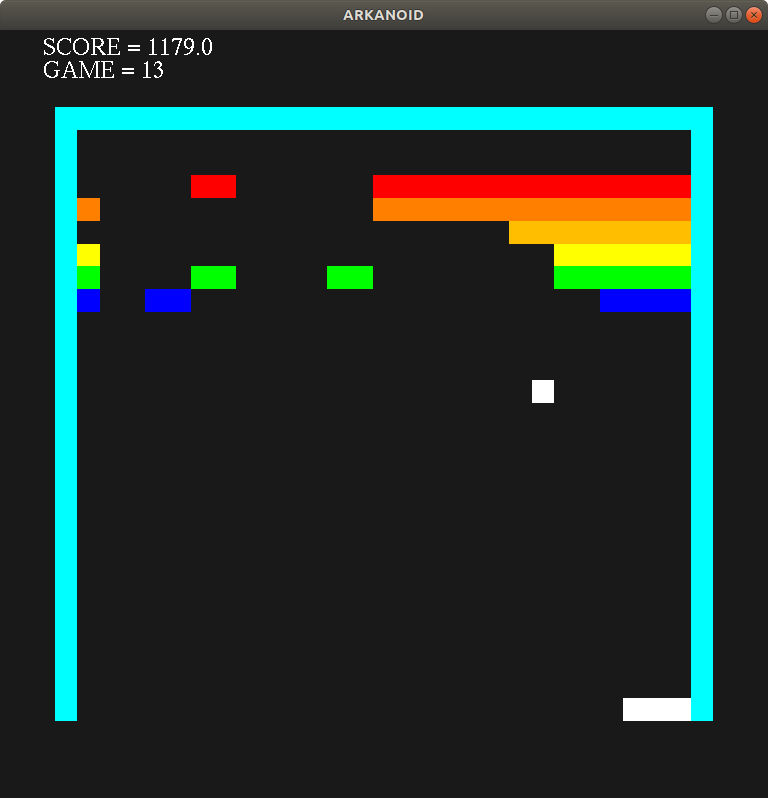
\includegraphics[scale=0.2]{../../pictures/arkanoid.png}
        \end{figure}

        \begin{itemize}
            \item neurons count {\bf 12 099}
            \item ant neurons count 250 000
            \item bee neurons count 960 000
        \end{itemize}

    \end{column}


\end{columns}




\end{frame}

\begin{frame}{\bf Applications}

\begin{itemize}
  \item self driving cars - Tesla model S
  \item healthcare, biomedical engineering - Cell in fluid
  \item voice search, control - Google, Amazon Echo
  \item machine translation - Google translator
  \item image recognition - Huawei Mate 10
  \item game bots, robotics - DeepMind, Boston Dynamics
\end{itemize}

\begin{columns}

    \begin{column}{0.33\textwidth}

      \begin{figure}
        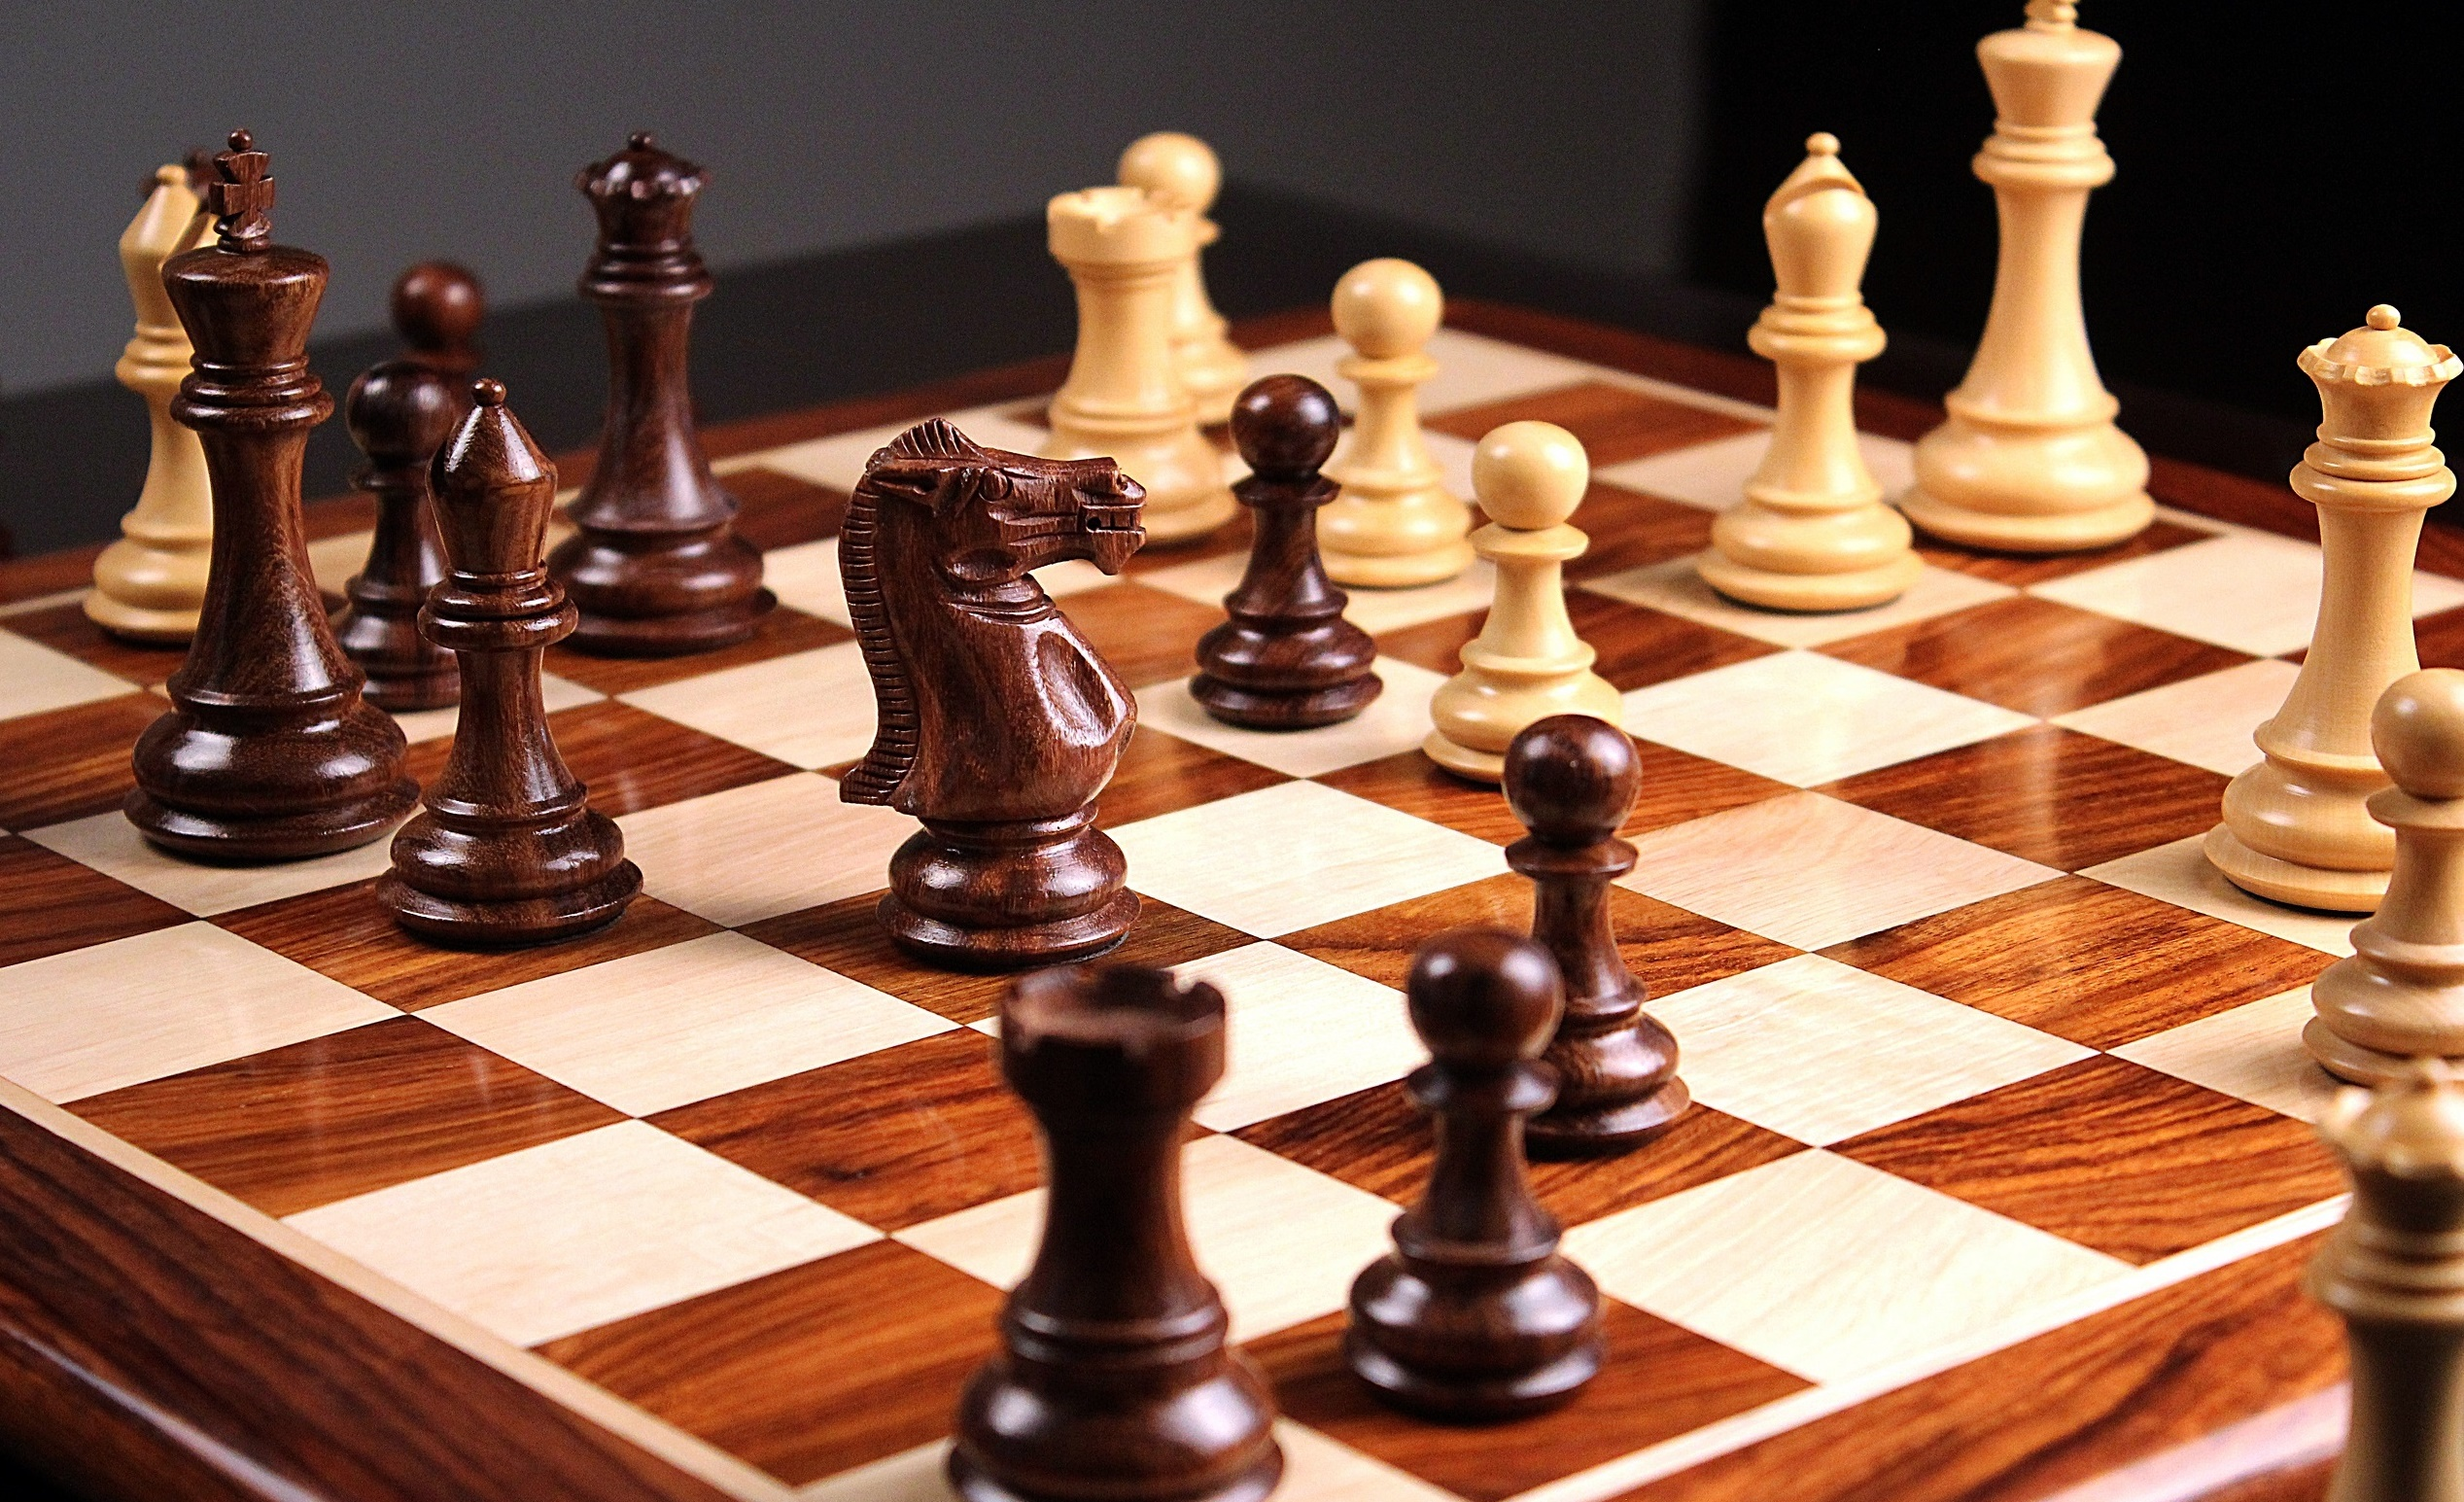
\includegraphics[scale=0.03]{../../pictures/chess.jpg}
      \end{figure}

    \end{column}

    \begin{column}{0.33\textwidth}  %%<--- here

      \begin{figure}
      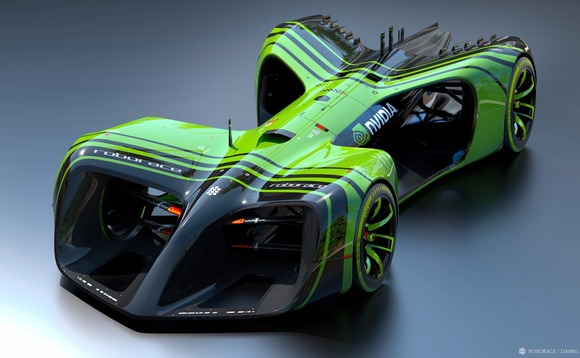
\includegraphics[scale=0.15]{../../pictures/nvidia_car.jpg}
      \end{figure}

    \end{column}


    \begin{column}{0.33\textwidth}  %%<--- here

        \begin{figure}
        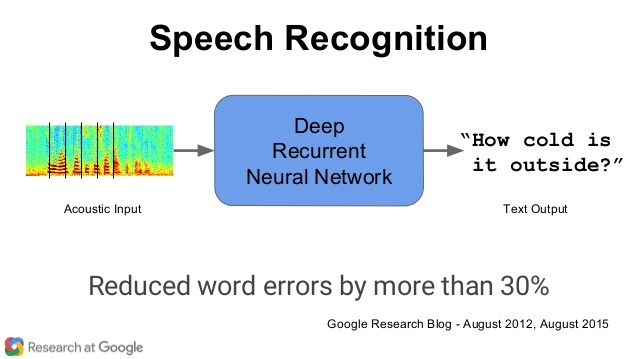
\includegraphics[scale=0.15]{../../pictures/speach_recognition.jpg}
        \end{figure}

    \end{column}

\end{columns}


\begin{figure}
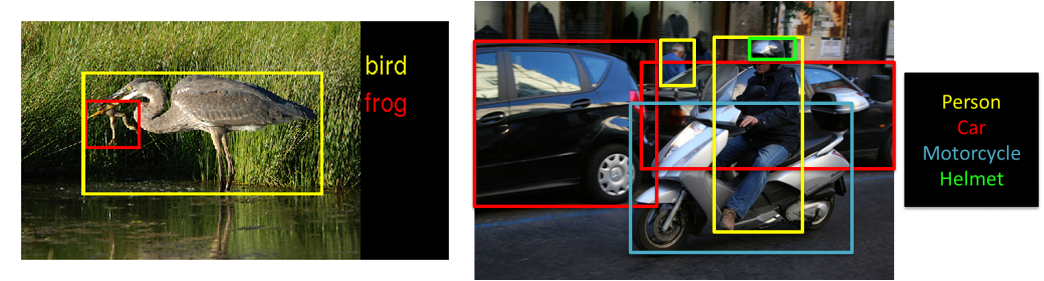
\includegraphics[scale=0.2]{../../pictures/image_recognition.png}
\end{figure}


\end{frame}


\begin{frame}{\bf Deep learning \footnotemark}

  \begin{figure}
    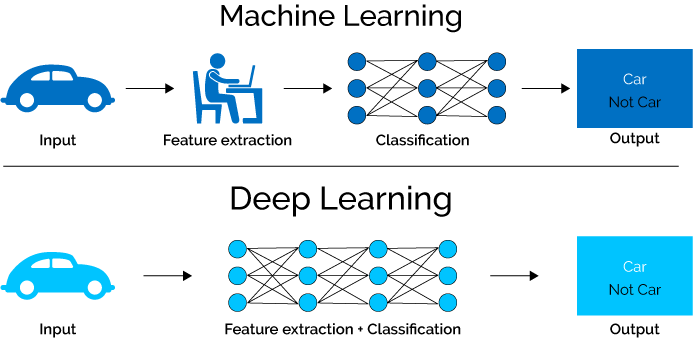
\includegraphics[scale=0.4]{../../pictures/end_to_end_learning.png}
  \end{figure}

\footnotetext[1]{\url {https://medium.com/datamob/clearing-the-buzzwords-in-machine-learning-e395ad73178b}}

\end{frame}



\begin{frame}{\bf Neural network}

\begin{columns}
    \begin{column}{0.4\textwidth}

    \begin{figure}
      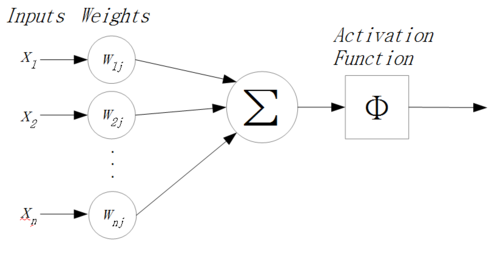
\includegraphics[scale=0.3]{../../diagrams/neuron_model.png}
    \end{figure}

    \end{column}

    \begin{column}{0.5\textwidth}  %%<--- here

    \begin{align*}
     y(X) = f(\sum_{i} X_iW_i + b)
    \end{align*}

    \end{column}

\end{columns}


  \begin{figure}
    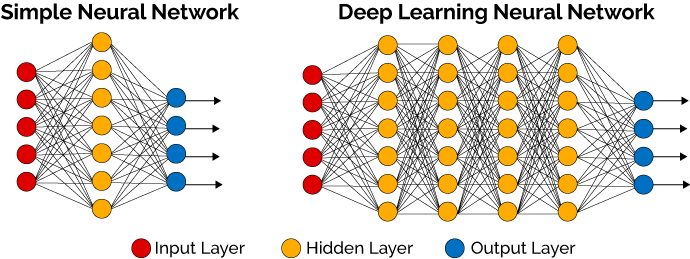
\includegraphics[scale=0.2]{../../diagrams/deep_nn.png}
  \end{figure}

  \begin{figure}
    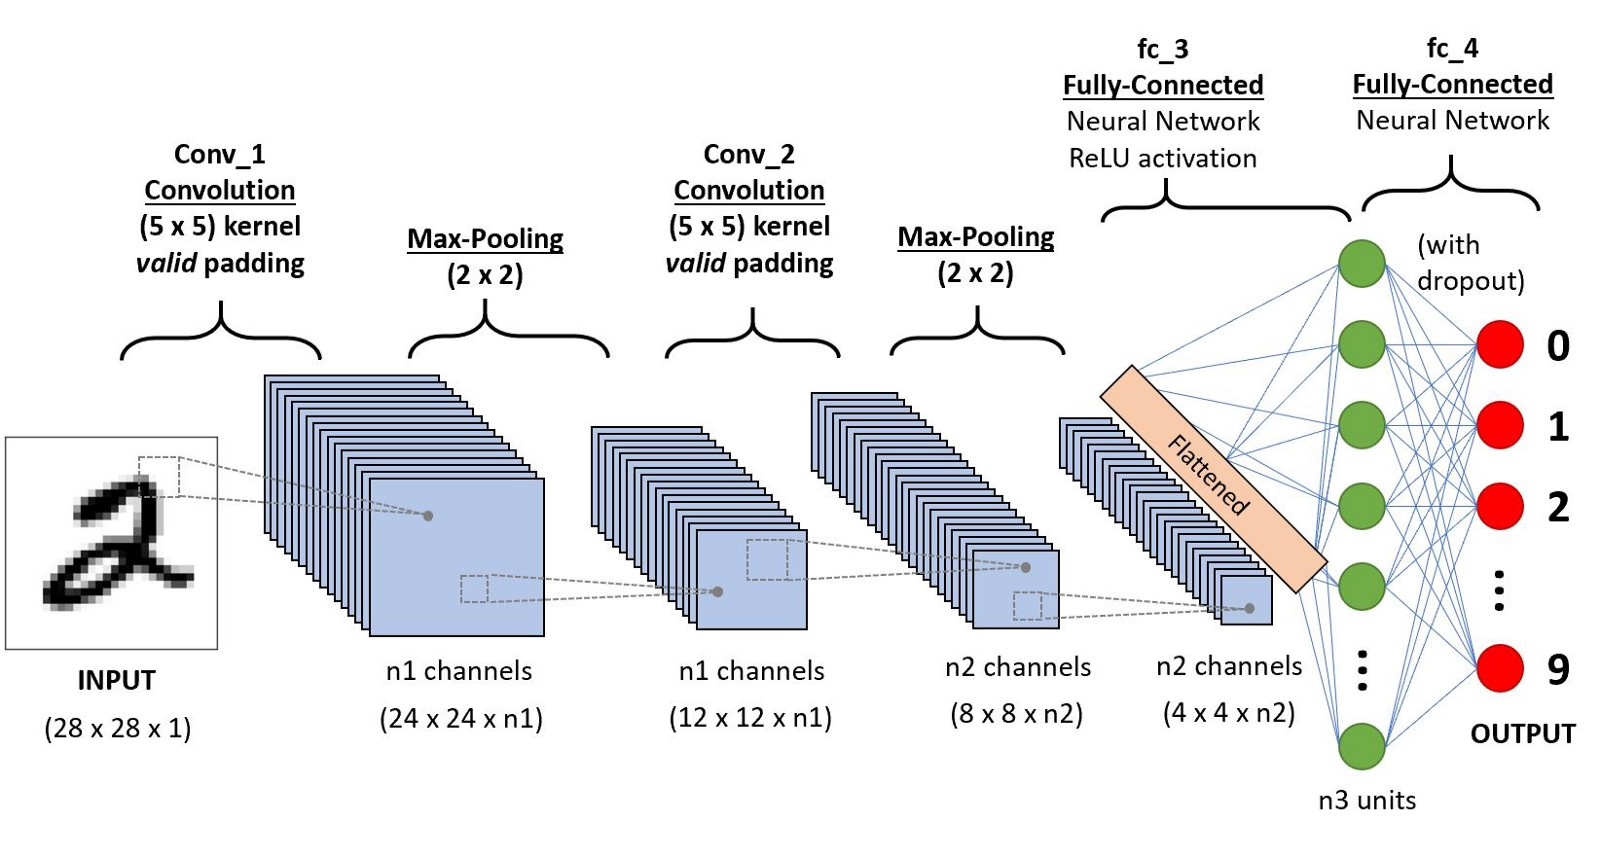
\includegraphics[scale=0.1]{../../pictures/cnn.jpg}
  \end{figure}

\end{frame}

\begin{frame}{\bf Deep neural network}

\begin{itemize}
  \item Old methods (before NN) - 2011, 25.8\%
  \item Convolutional, AlexNet - 2012, 16.4\%
  \item Google inception - 2013, 6.7\%
  \item Microsoft ResNet - 2015, 6.1\%
  \item DenseNet - 2018, 5.17\%
\end{itemize}

\begin{itemize}

    \item CNN
    \begin{figure}
      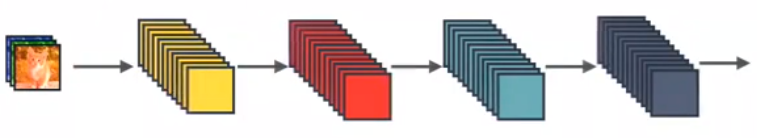
\includegraphics[scale=0.15]{../../diagrams/dnn_conv.png}
    \end{figure}

    \item ResNET
    \begin{figure}
      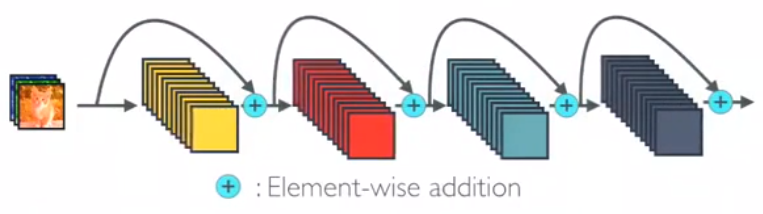
\includegraphics[scale=0.15]{../../diagrams/dnn_resnet.png}
    \end{figure}

    \item DenseNet
    \begin{figure}
      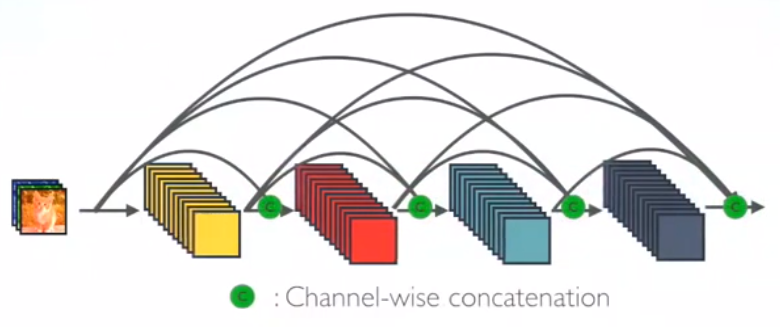
\includegraphics[scale=0.15]{../../diagrams/dnn_densenet.png}
    \end{figure}

\end{itemize}

\end{frame}




\begin{frame}{\bf My research}

\begin{itemize}
  \item Robotics - hobby
  \item Red blood cells trajectory prediction
  \item Deep reinforcement learning
\end{itemize}

\end{frame}


\begin{frame}{\bf Robotics - line follower}

Curve shape classification

\begin{columns}

    \begin{column}{0.5\textwidth}

    \begin{itemize}
      \item stm32f303 (72MHz), stm32f746 (216MHz)
      \item 8x 500nm line sensors
      \item pololu motors, 1:30
      \item network input : 8 last line sensors results (8x8 matrix)
      \item response 4..5ms
    \end{itemize}

        \begin{figure}
          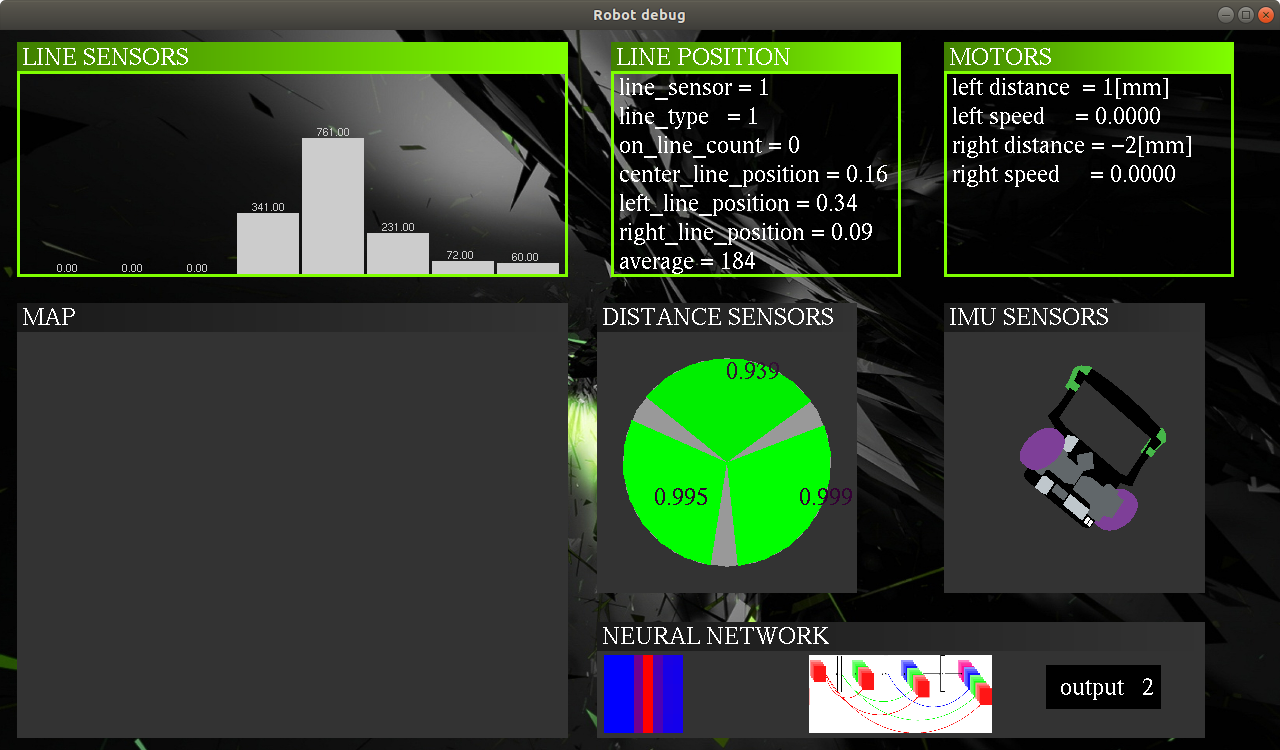
\includegraphics[scale=0.1]{../../pictures/robot_debug_app.png}
        \end{figure}

    \end{column}

    \begin{column}{0.5\textwidth}  %%<--- here

        \begin{figure}
          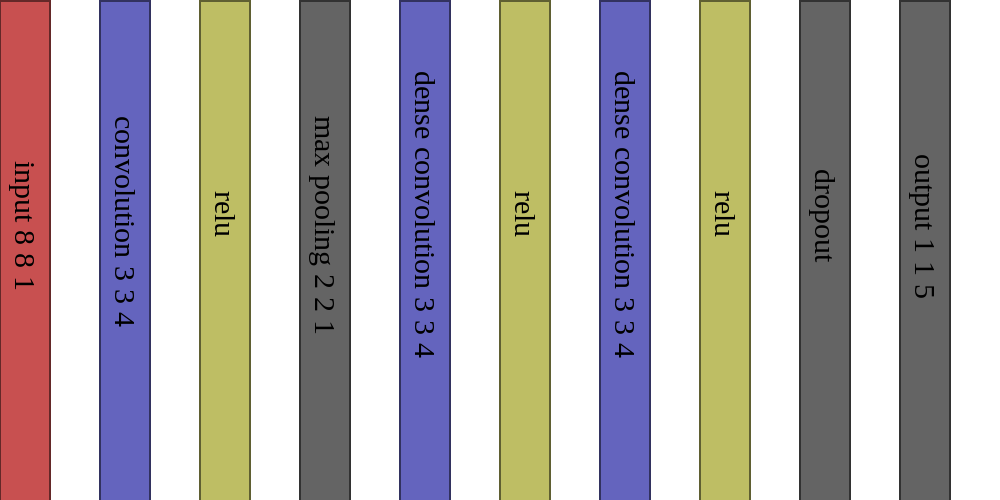
\includegraphics[scale=0.18]{../../diagrams/line_following_net.png}
        \end{figure}

        \begin{figure}
          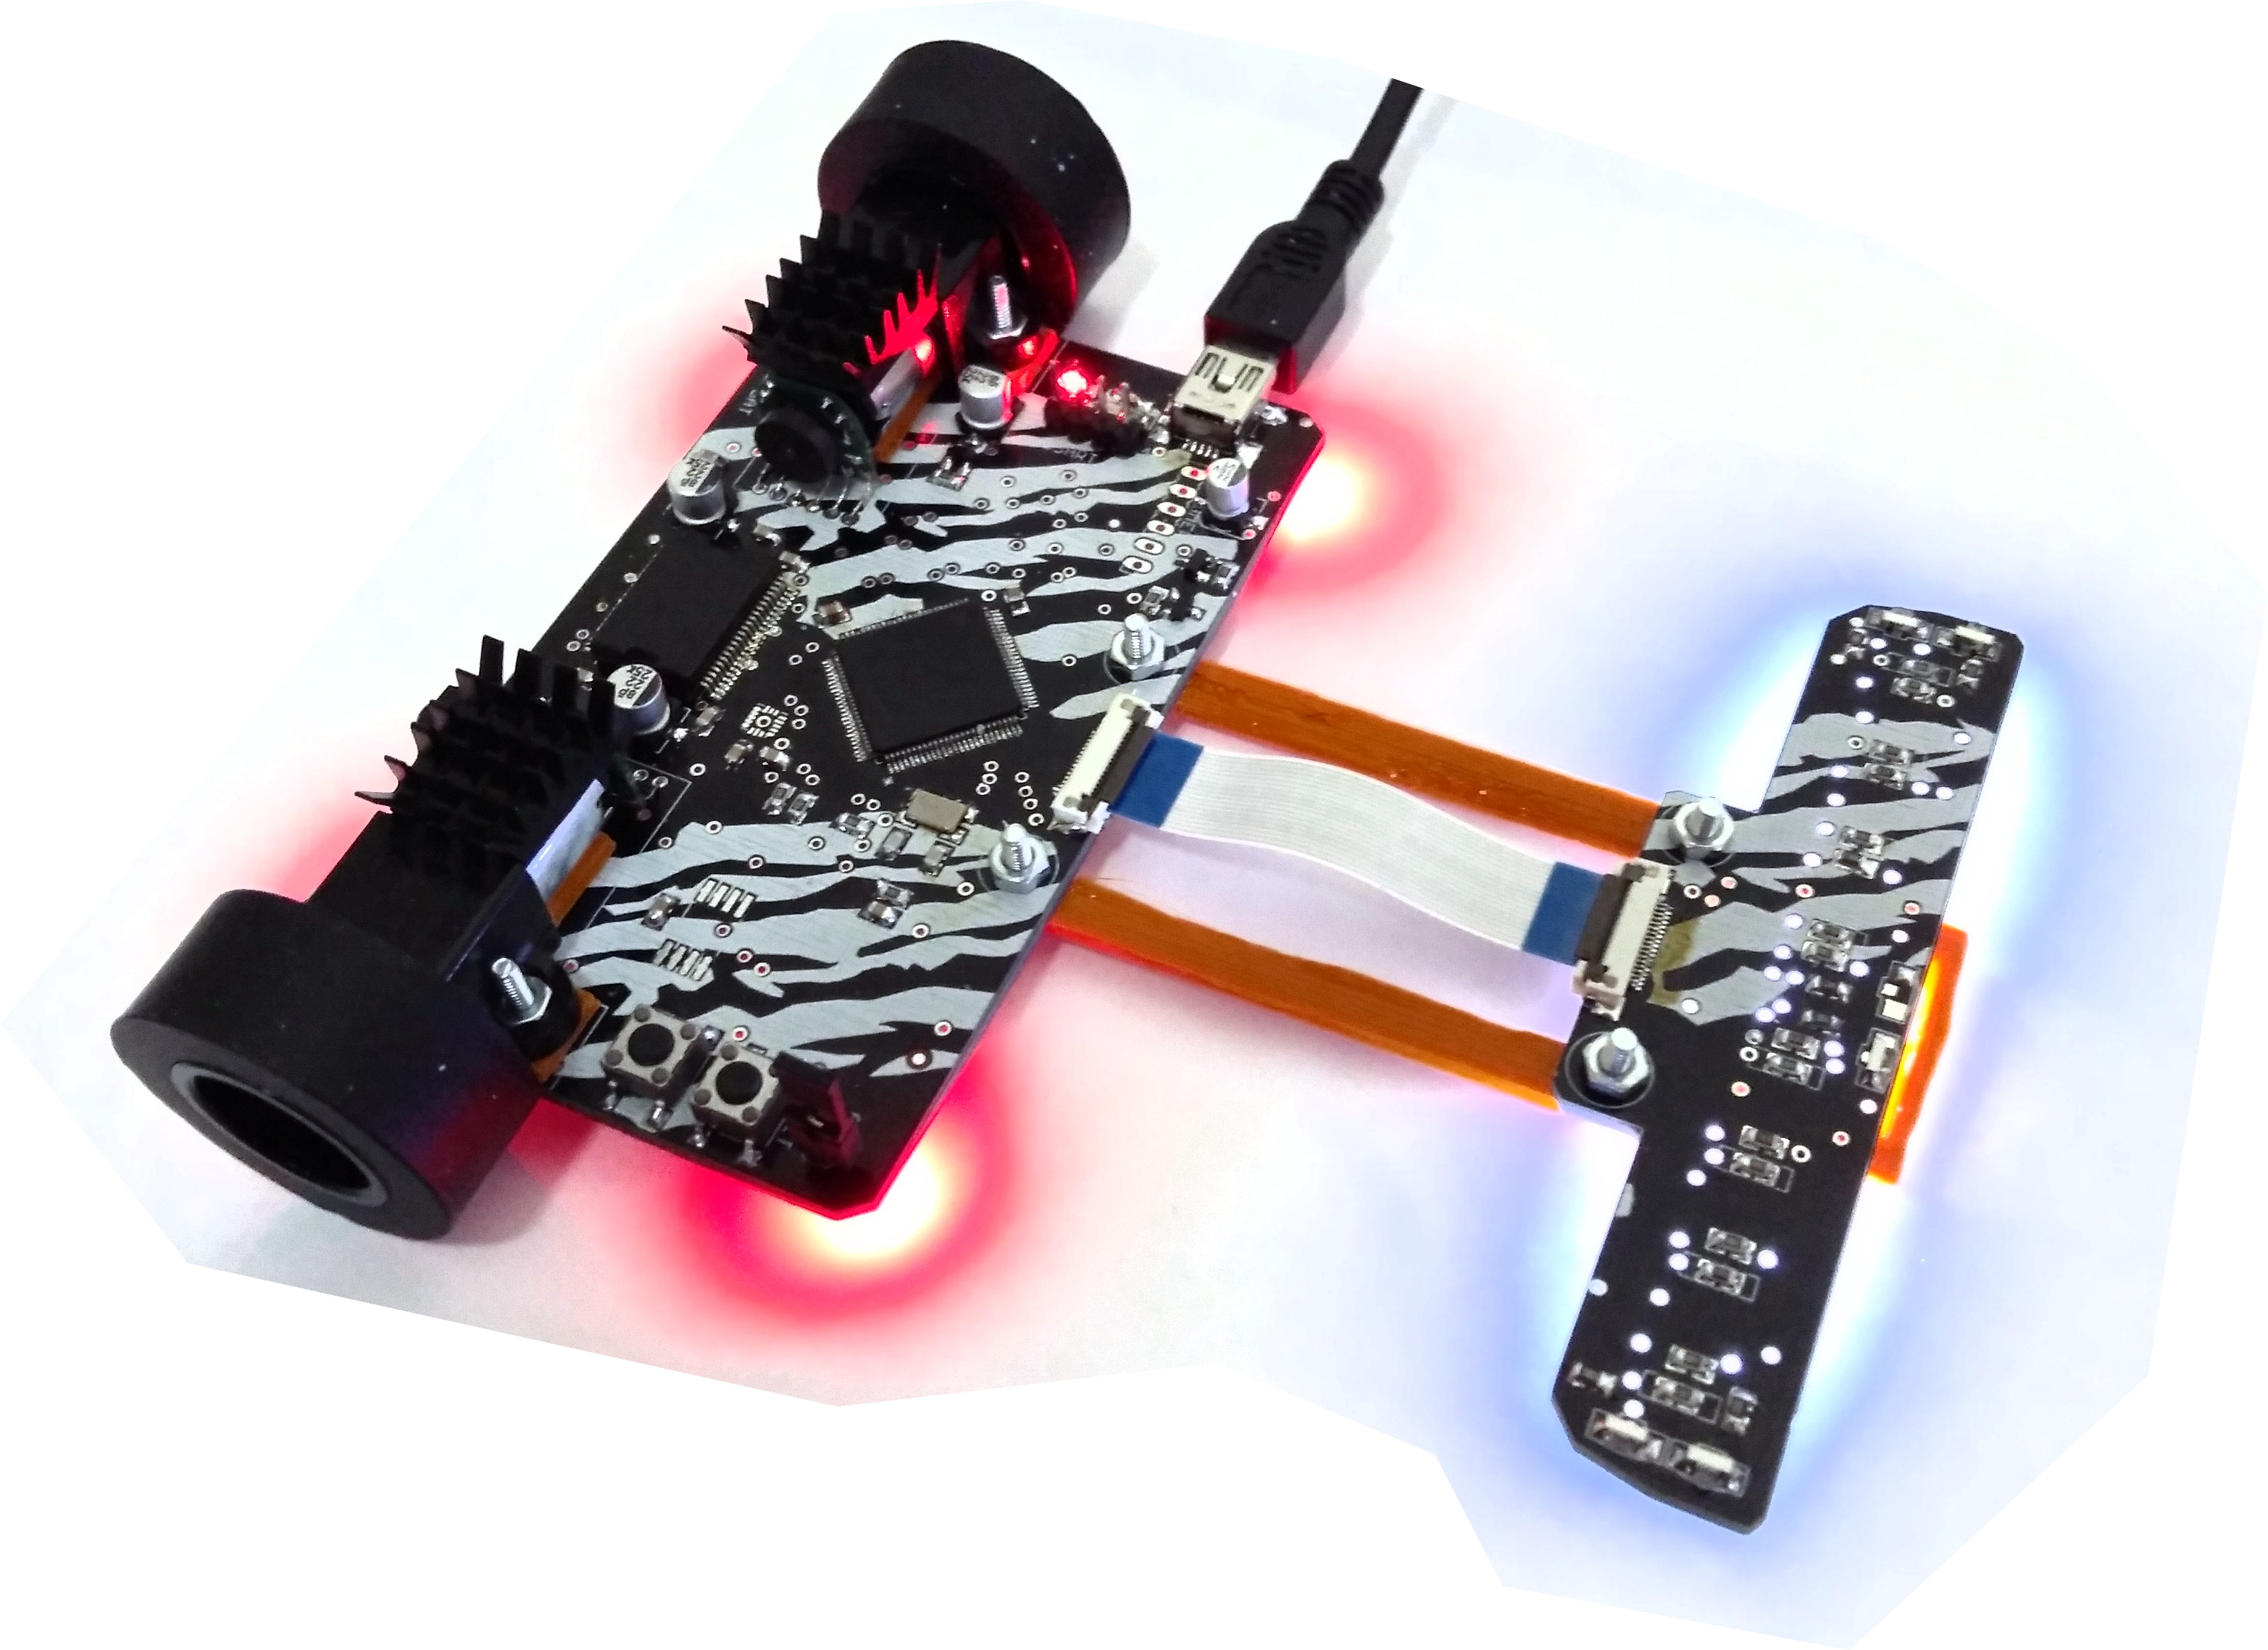
\includegraphics[scale=0.04]{../../pictures/robot_ascender.jpg}
        \end{figure}

    \end{column}

\end{columns}


\end{frame}


\begin{frame}{\bf Red blood cells trajectory prediction}
Research group Cell in fluid
(Mgr. Katarína Jasenčáková, PhD thesis)

\begin{itemize}
  \item train DNN to predict RBC trajectory from past
  \item 15 conv layers network (6hours training on GTX1080ti)
  \item input : RBC position + 7 past frames + other cells position
  \item output: RBC predicted velocity
\end{itemize}

\begin{figure}
  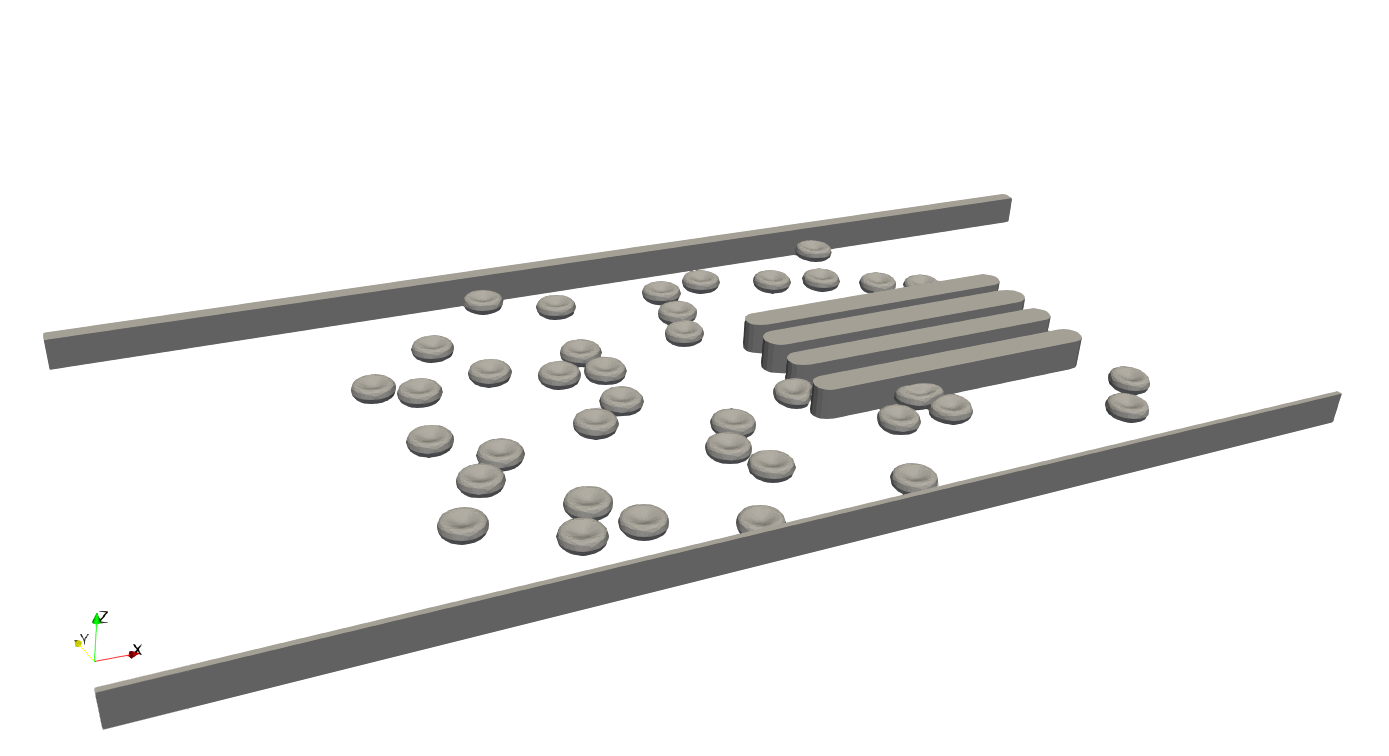
\includegraphics[scale=0.08]{../../pictures/rbc_channel.png}
\end{figure}


\begin{figure}
  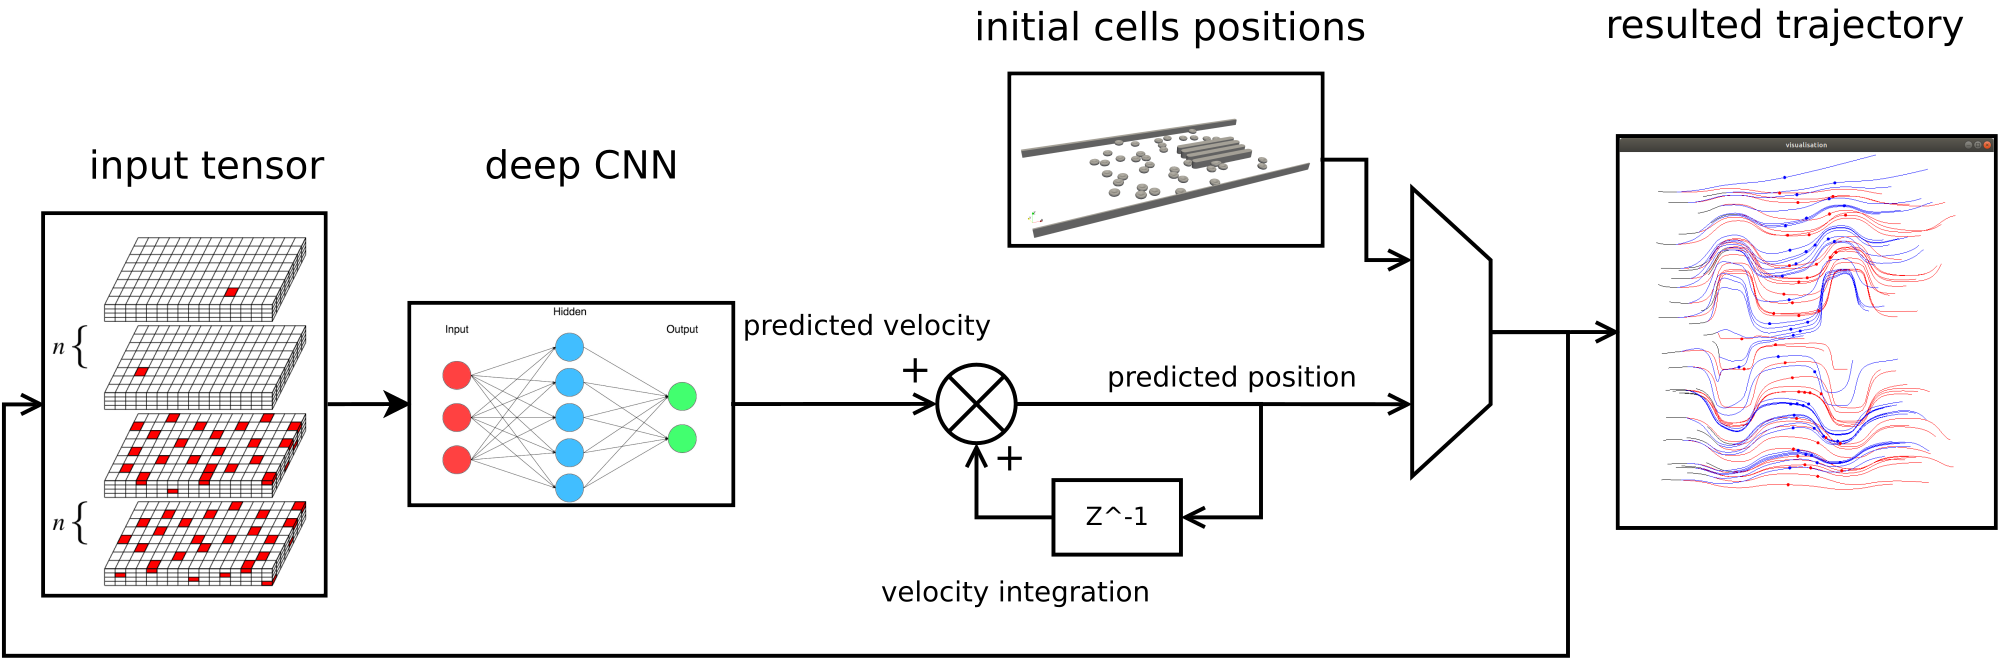
\includegraphics[scale=0.12]{../../diagrams/cells_prediction_velocity_integration.png}
\end{figure}


\end{frame}


\begin{frame}{\bf Networks}


{\fontsize{5.2}{7}\selectfont

\begin{table}[]
\begin{tabular}{|l|l|l|l|l|l|l|l|l|}
\hline
\textbf{layer} & \textbf{net 0}                 & \textbf{net 1}                                                                 & \textbf{net 2}                                                                      & \textbf{net 3}                                                                      & \textbf{net 4}                                                                      & \textbf{net 5}                                                                      & \textbf{net 6}                                                                      & \textbf{net 7}                                                                      \\ \hline
0              & \cellcolor[HTML]{67FD9A}fc 256 & \cellcolor[HTML]{34CDF9}\begin{tabular}[c]{@{}l@{}}conv \\ 3x3x32\end{tabular} & \cellcolor[HTML]{FD6864}\begin{tabular}[c]{@{}l@{}}dense conv\\  3x3x8\end{tabular} & \cellcolor[HTML]{FD6864}\begin{tabular}[c]{@{}l@{}}dense conv\\  3x3x8\end{tabular} & \cellcolor[HTML]{FD6864}\begin{tabular}[c]{@{}l@{}}dense conv\\  3x3x8\end{tabular} & \cellcolor[HTML]{FD6864}\begin{tabular}[c]{@{}l@{}}dense conv\\  3x3x8\end{tabular} & \cellcolor[HTML]{FD6864}\begin{tabular}[c]{@{}l@{}}dense conv\\  3x3x8\end{tabular} & \cellcolor[HTML]{FD6864}\begin{tabular}[c]{@{}l@{}}dense conv\\  3x3x8\end{tabular} \\ \hline
1              & \cellcolor[HTML]{67FD9A}fc 64  & \cellcolor[HTML]{67FD9A}fc 64                                                  & \cellcolor[HTML]{FD6864}\begin{tabular}[c]{@{}l@{}}dense conv\\  3x3x8\end{tabular} & \cellcolor[HTML]{FD6864}\begin{tabular}[c]{@{}l@{}}dense conv\\  3x3x8\end{tabular} & \cellcolor[HTML]{FD6864}\begin{tabular}[c]{@{}l@{}}dense conv\\  3x3x8\end{tabular} & \cellcolor[HTML]{FD6864}\begin{tabular}[c]{@{}l@{}}dense conv\\  3x3x8\end{tabular} & \cellcolor[HTML]{FD6864}\begin{tabular}[c]{@{}l@{}}dense conv\\  3x3x8\end{tabular} & \cellcolor[HTML]{FD6864}\begin{tabular}[c]{@{}l@{}}dense conv\\  3x3x8\end{tabular} \\ \hline
2              & \cellcolor[HTML]{67FD9A}fc 32  & \cellcolor[HTML]{67FD9A}fc 32                                                  & \cellcolor[HTML]{FD6864}\begin{tabular}[c]{@{}l@{}}dense conv\\  3x3x8\end{tabular} & \cellcolor[HTML]{FD6864}\begin{tabular}[c]{@{}l@{}}dense conv\\  3x3x8\end{tabular} & \cellcolor[HTML]{FD6864}\begin{tabular}[c]{@{}l@{}}dense conv\\  3x3x8\end{tabular} & \cellcolor[HTML]{FD6864}\begin{tabular}[c]{@{}l@{}}dense conv\\  3x3x8\end{tabular} & \cellcolor[HTML]{FD6864}\begin{tabular}[c]{@{}l@{}}dense conv\\  3x3x8\end{tabular} & \cellcolor[HTML]{FD6864}\begin{tabular}[c]{@{}l@{}}dense conv\\  3x3x8\end{tabular} \\ \hline
3              & \cellcolor[HTML]{67FD9A}fc 3   & \cellcolor[HTML]{67FD9A}fc 3                                                   & \cellcolor[HTML]{FD6864}\begin{tabular}[c]{@{}l@{}}dense conv\\  3x3x8\end{tabular} & \cellcolor[HTML]{FD6864}\begin{tabular}[c]{@{}l@{}}dense conv\\  3x3x8\end{tabular} & \cellcolor[HTML]{FD6864}\begin{tabular}[c]{@{}l@{}}dense conv\\  3x3x8\end{tabular} & \cellcolor[HTML]{FD6864}\begin{tabular}[c]{@{}l@{}}dense conv\\  3x3x8\end{tabular} & \cellcolor[HTML]{FD6864}\begin{tabular}[c]{@{}l@{}}dense conv\\  3x3x8\end{tabular} & \cellcolor[HTML]{FD6864}\begin{tabular}[c]{@{}l@{}}dense conv\\  3x3x8\end{tabular} \\ \hline
4              &                                &                                                                                & \cellcolor[HTML]{34CDF9}conv 1x1x32                                                 & \cellcolor[HTML]{34CDF9}conv 1x1x16                                                 & \cellcolor[HTML]{34CDF9}conv 1x1x32                                                 & \cellcolor[HTML]{34CDF9}conv 1x1x16                                                 & \cellcolor[HTML]{34CDF9}conv 1x1x16                                                 & \cellcolor[HTML]{34CDF9}conv 1x1x32                                                 \\ \hline
5              &                                &                                                                                & \cellcolor[HTML]{67FD9A}fc 3                                                        & \cellcolor[HTML]{FD6864}\begin{tabular}[c]{@{}l@{}}dense conv\\  3x3x8\end{tabular} & \cellcolor[HTML]{67FD9A}fc 3                                                        & \cellcolor[HTML]{FD6864}\begin{tabular}[c]{@{}l@{}}dense conv\\  3x3x8\end{tabular} & \cellcolor[HTML]{FD6864}\begin{tabular}[c]{@{}l@{}}dense conv\\  3x3x8\end{tabular} & \cellcolor[HTML]{FD6864}\begin{tabular}[c]{@{}l@{}}dense conv\\  3x3x8\end{tabular} \\ \hline
6              &                                &                                                                                &                                                                                     & \cellcolor[HTML]{FD6864}\begin{tabular}[c]{@{}l@{}}dense conv\\  3x3x8\end{tabular} &                                                                                     & \cellcolor[HTML]{FD6864}\begin{tabular}[c]{@{}l@{}}dense conv\\  3x3x8\end{tabular} & \cellcolor[HTML]{FD6864}\begin{tabular}[c]{@{}l@{}}dense conv\\  3x3x8\end{tabular} & \cellcolor[HTML]{FD6864}\begin{tabular}[c]{@{}l@{}}dense conv\\  3x3x8\end{tabular} \\ \hline
7              &                                &                                                                                &                                                                                     & \cellcolor[HTML]{FD6864}\begin{tabular}[c]{@{}l@{}}dense conv\\  3x3x8\end{tabular} &                                                                                     & \cellcolor[HTML]{FD6864}\begin{tabular}[c]{@{}l@{}}dense conv\\  3x3x8\end{tabular} & \cellcolor[HTML]{FD6864}\begin{tabular}[c]{@{}l@{}}dense conv\\  3x3x8\end{tabular} & \cellcolor[HTML]{FD6864}\begin{tabular}[c]{@{}l@{}}dense conv\\  3x3x8\end{tabular} \\ \hline
8              &                                &                                                                                &                                                                                     & \cellcolor[HTML]{FD6864}\begin{tabular}[c]{@{}l@{}}dense conv\\  3x3x8\end{tabular} &                                                                                     & \cellcolor[HTML]{FD6864}\begin{tabular}[c]{@{}l@{}}dense conv\\  3x3x8\end{tabular} & \cellcolor[HTML]{FD6864}\begin{tabular}[c]{@{}l@{}}dense conv\\  3x3x8\end{tabular} & \cellcolor[HTML]{FD6864}\begin{tabular}[c]{@{}l@{}}dense conv\\  3x3x8\end{tabular} \\ \hline
9              &                                &                                                                                &                                                                                     & \cellcolor[HTML]{34CDF9}conv 1x1x32                                                 &                                                                                     & \cellcolor[HTML]{34CDF9}conv 1x1x32                                                 & \cellcolor[HTML]{34CDF9}conv 1x1x16                                                 & \cellcolor[HTML]{34CDF9}conv 1x1x32                                                 \\ \hline
10             &                                &                                                                                &                                                                                     & \cellcolor[HTML]{67FD9A}fc 3                                                        &                                                                                     & \cellcolor[HTML]{67FD9A}fc 3                                                        & \cellcolor[HTML]{FD6864}\begin{tabular}[c]{@{}l@{}}dense conv\\  3x3x8\end{tabular} & \cellcolor[HTML]{FD6864}\begin{tabular}[c]{@{}l@{}}dense conv\\  3x3x8\end{tabular} \\ \hline
11             &                                &                                                                                &                                                                                     &                                                                                     &                                                                                     &                                                                                     & \cellcolor[HTML]{FD6864}\begin{tabular}[c]{@{}l@{}}dense conv\\  3x3x8\end{tabular} & \cellcolor[HTML]{FD6864}\begin{tabular}[c]{@{}l@{}}dense conv\\  3x3x8\end{tabular} \\ \hline
12             &                                &                                                                                &                                                                                     &                                                                                     &                                                                                     &                                                                                     & \cellcolor[HTML]{FD6864}\begin{tabular}[c]{@{}l@{}}dense conv\\  3x3x8\end{tabular} & \cellcolor[HTML]{FD6864}\begin{tabular}[c]{@{}l@{}}dense conv\\  3x3x8\end{tabular} \\ \hline
13             &                                &                                                                                &                                                                                     &                                                                                     &                                                                                     &                                                                                     & \cellcolor[HTML]{FD6864}\begin{tabular}[c]{@{}l@{}}dense conv\\  3x3x8\end{tabular} & \cellcolor[HTML]{FD6864}\begin{tabular}[c]{@{}l@{}}dense conv\\  3x3x8\end{tabular} \\ \hline
14             &                                &                                                                                &                                                                                     &                                                                                     &                                                                                     &                                                                                     & \cellcolor[HTML]{34CDF9}conv 1x1x32                                                 & \cellcolor[HTML]{34CDF9}conv 1x1x64                                                 \\ \hline
15             &                                &                                                                                &                                                                                     &                                                                                     &                                                                                     &                                                                                     & \cellcolor[HTML]{67FD9A}fc 3                                                        & \cellcolor[HTML]{67FD9A}fc 3                                                        \\ \hline
\end{tabular}
\end{table}
}

\end{frame}

\begin{frame}{\bf Results}


\begin{columns}

    \begin{column}{0.5\textwidth}

        \includemovie[
          poster,
          autoplay,
          externalviewer,
          inline=false,
          text={\small(video)}
        ]{4cm}{4cm}{../../video/cells_trajectory.mp4}

    \end{column}

    \begin{column}{0.5\textwidth}  %%<--- here

        \begin{figure}
          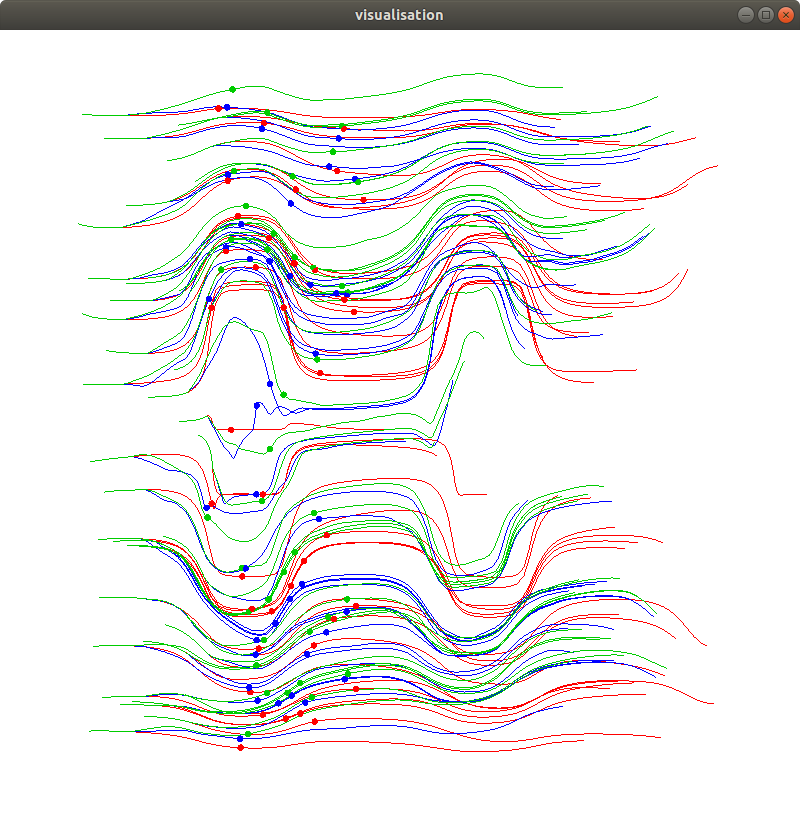
\includegraphics[scale=0.2]{../../diagrams/rbc_deep_network_6_7.png}
        \end{figure}

    \end{column}

\end{columns}

\end{frame}


\begin{frame}{\bf Results}

\begin{table}[]
\begin{tabular}{|l|llll|}
\hline
\textbf{ID} & \multicolumn{1}{c}{}                                                                  & \multicolumn{1}{c}{}                                                                   & \multicolumn{1}{c}{\textbf{total error}}                                             & \multicolumn{1}{c|}{}                                                                            \\ \hline
            & \multicolumn{1}{c|}{\textbf{\begin{tabular}[c]{@{}c@{}}mean\\ {[}um{]}\end{tabular}}} & \multicolumn{1}{c|}{\textbf{\begin{tabular}[c]{@{}c@{}}sigma\\ {[}um{]}\end{tabular}}} & \multicolumn{1}{c|}{\textbf{\begin{tabular}[c]{@{}c@{}}rms\\ {[}um{]}\end{tabular}}} & \multicolumn{1}{c|}{\textbf{\begin{tabular}[c]{@{}c@{}}rms \\ relative\\ {[}\%{]}\end{tabular}}} \\ \hline
\textbf{0}  & \multicolumn{1}{l|}{{\color[HTML]{333333} -9.8}}                                      & \multicolumn{1}{l|}{{\color[HTML]{333333} 38.88}}                                      & \multicolumn{1}{l|}{{\color[HTML]{333333} 40.1}}                                     & {\color[HTML]{333333} 7.23}                                                                      \\ \hline
\textbf{1}  & \multicolumn{1}{l|}{{\color[HTML]{FE0000} \textbf{-36.99}}}                           & \multicolumn{1}{l|}{{\color[HTML]{FE0000} \textbf{215.02}}}                            & \multicolumn{1}{l|}{{\color[HTML]{FE0000} \textbf{218.18}}}                          & {\color[HTML]{FE0000} \textbf{39.32}}                                                            \\ \hline
\textbf{2}  & \multicolumn{1}{l|}{{\color[HTML]{333333} -3.85}}                                     & \multicolumn{1}{l|}{{\color[HTML]{333333} 23.11}}                                      & \multicolumn{1}{l|}{{\color[HTML]{333333} 23.43}}                                    & {\color[HTML]{333333} 4.22}                                                                      \\ \hline
\textbf{3}  & \multicolumn{1}{l|}{{\color[HTML]{333333} -0.32}}                                     & \multicolumn{1}{l|}{{\color[HTML]{333333} 16.09}}                                      & \multicolumn{1}{l|}{{\color[HTML]{333333} 16.09}}                                    & {\color[HTML]{333333} 2.9}                                                                       \\ \hline
\textbf{4}  & \multicolumn{1}{l|}{{\color[HTML]{333333} -1.26}}                                     & \multicolumn{1}{l|}{{\color[HTML]{333333} 11.44}}                                      & \multicolumn{1}{l|}{{\color[HTML]{333333} 11.51}}                                    & {\color[HTML]{333333} 2.07}                                                                      \\ \hline
\textbf{5}  & \multicolumn{1}{l|}{{\color[HTML]{32CB00} \textbf{-0.25}}}                            & \multicolumn{1}{l|}{{\color[HTML]{32CB00} \textbf{11.27}}}                             & \multicolumn{1}{l|}{{\color[HTML]{32CB00} \textbf{11.28}}}                           & {\color[HTML]{32CB00} \textbf{2.03}}                                                             \\ \hline
\textbf{6}  & \multicolumn{1}{l|}{{\color[HTML]{333333} -0.85}}                                     & \multicolumn{1}{l|}{{\color[HTML]{333333} 12.26}}                                      & \multicolumn{1}{l|}{{\color[HTML]{333333} 12.29}}                                    & {\color[HTML]{333333} 2.22}                                                                      \\ \hline
\textbf{7}  & \multicolumn{1}{l|}{{\color[HTML]{333333} -1.67}}                                     & \multicolumn{1}{l|}{{\color[HTML]{333333} 11.9}}                                       & \multicolumn{1}{l|}{{\color[HTML]{333333} 12.02}}                                    & {\color[HTML]{333333} 2.17}                                                                      \\ \hline
\end{tabular}
\end{table}

\end{frame}



\begin{frame}{\bf Playing GO}


  \begin{columns}
  \begin{column}{0.5\textwidth}

    \begin{figure}[!htb]
      \centering
      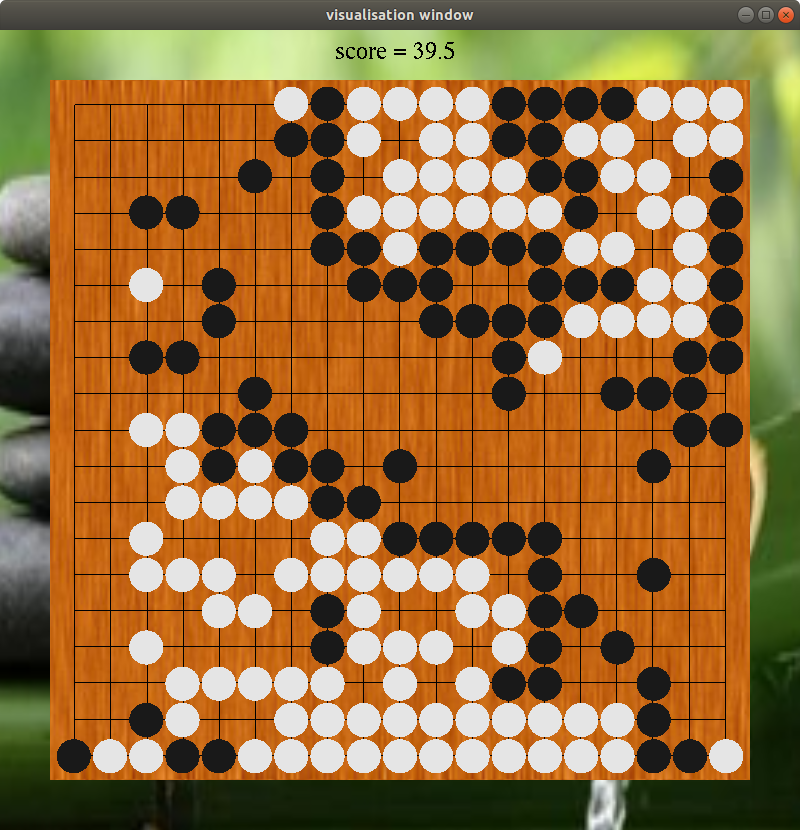
\includegraphics[scale=0.18]{../../pictures/go_board.png}
    \end{figure}


  \end{column}
  \begin{column}{0.5\textwidth}  %%<--- here

    \scriptsize
    {
      \begin{itemize}
        \item {\bf supervised training} - train game using Masters games
        \item {\bf reinforcement learning} - let play two networks against each other
      \end{itemize}
    }
  \end{column}
  \end{columns}

\end{frame}

\begin{frame}{\bf Network architecture}
we need to go much deeper for GO
\begin{itemize}
  \item {\bf 28, 35 layers} \\ dense blocks + feature pooling layer
  \item {\bf input} \\ 4 matrices $19x19$: black stones, white stones, empty fields, active player
  \item {\bf output} \\ recommended moves 19x19 + 1 for pass = 362 outputs

\end{itemize}

  \begin{figure}[!htb]
    \centering
    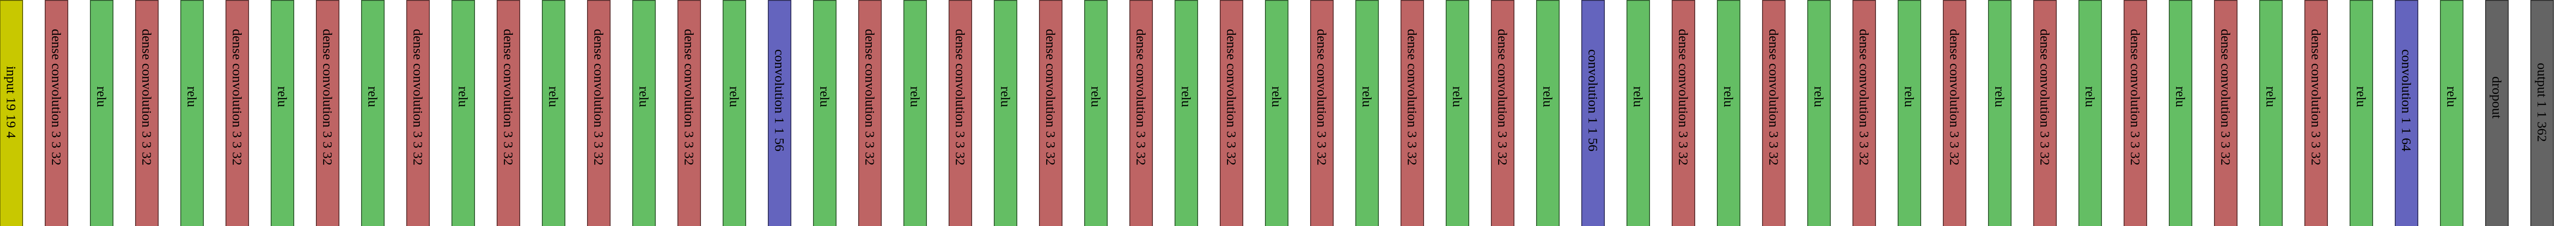
\includegraphics[scale=0.06]{../../diagrams/net_go_1_28_layers.png}
  \end{figure}

  \begin{figure}[!htb]
    \centering
    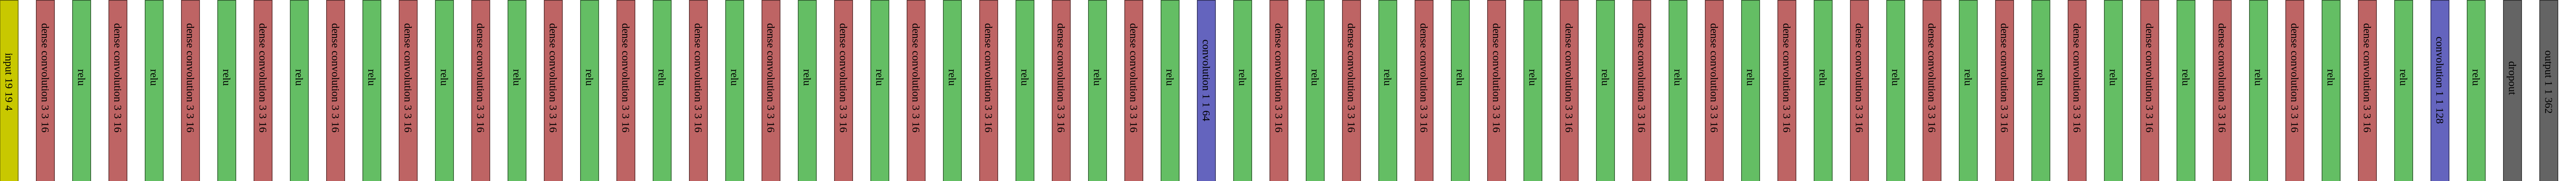
\includegraphics[scale=0.06]{../../diagrams/net_go_5_35_layers.png}
  \end{figure}

\end{frame}


\begin{frame}{\bf Reinforcement learning}

\begin{itemize}
  \item learn from punishment and rewards
  \item learn to play a game with unknown rules
  \item obtain {\bf state}, $s$
  \item choose {\bf action}, $a$
  \item {\bf execute} action
  \item obtain {\bf reward}, $R$
  \item learn from {\bf experiences}, $Q(s, a) = R + \gamma \max \limits_{\alpha'} Q(s', \alpha')$
\end{itemize}



\begin{columns}
\begin{column}{0.5\textwidth}

\begin{align*}
Q(s, a) \approx \hat{Q}(s, a; w)
\end{align*}

\end{column}
\begin{column}{0.5\textwidth}  %%<--- here
  \begin{figure}
    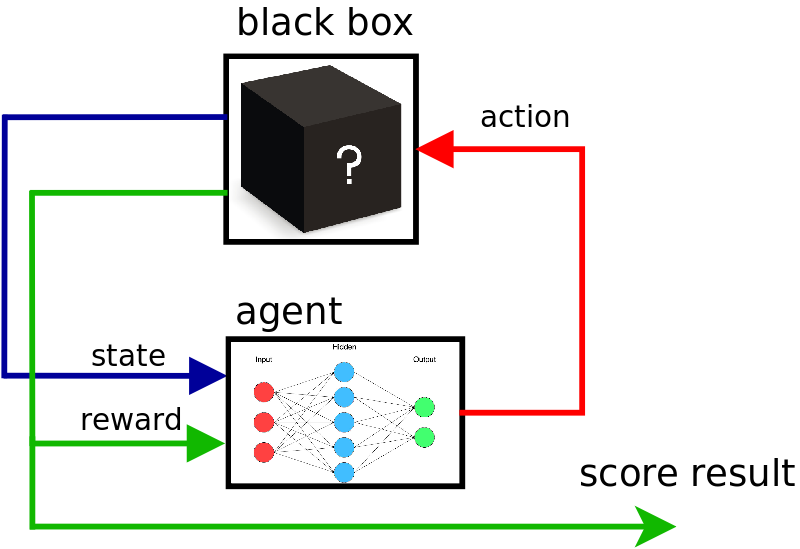
\includegraphics[scale=0.28]{../../diagrams/rl_mechanism.png}
  \end{figure}
\end{column}
\end{columns}

\end{frame}



\begin{frame}{\bf Q\&A}

\begin{figure}
  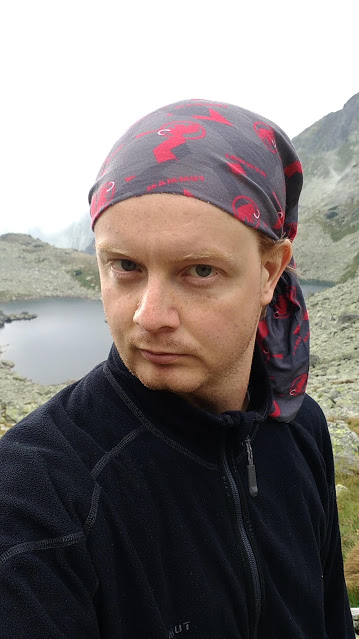
\includegraphics[scale=0.25]{../../pictures/me.jpg}
\end{figure}

\centering {
michal chovanec (michal.nand@gmail.com)
\url{www.youtube.com/channel/UCzVvP2ou8v3afNiVrPAHQGg}
}

\centering {
github
\url{https://github.com/michalnand}
}

\end{frame}


\end{document}
